\documentclass{beamer}


\usepackage[english]{babel}
\usepackage{xcolor}
\usepackage{xmpmulti}
\usepackage{amsmath}
\usepackage{dsfont}
\usepackage{multicol}
\usepackage{tikz}
\usepackage{eucal}
\usetikzlibrary{positioning,angles,quotes}
\usepackage{url}
\usepackage{graphicx}
\usepackage{cmbright}
\usepackage{framed}
\usepackage{algorithm}
%\usepackage[]{algorithm2e}
%\usepackage{algpseudocode}

\usepackage[noend]{algpseudocode}

\usetikzlibrary{pgfplots.groupplots,arrows.meta,shadows,positioning,angles,quotes}
\usetikzlibrary{matrix,chains,positioning,decorations.pathreplacing,arrows}
\usepackage{tikz}
\usetikzlibrary{shapes.geometric}
\usetikzlibrary{positioning}
\usepackage{pgfplots}



%\input{epgfplotslibrary{groupplots}
\usetikzlibrary{pgfplots.groupplots,arrows.meta,shadows,positioning,angles,quotes}
\usetikzlibrary{matrix,chains,positioning,decorations.pathreplacing,arrows}



\DeclareMathOperator*{\argmax}{arg\,max}
\def\checkmark{\tikz\fill[scale=0.4](0,.35) -- (.25,0) -- (1,.7) -- (.25,.15) -- cycle;} 

\definecolor{Maroon}{cmyk}{0, 0.87, 0.68, 0.32}
\definecolor{RoyalBlue}{cmyk}{1, 0.50, 0, 0}
\definecolor{skymagenta}{rgb}{0.81, 0.44, 0.69}

\newenvironment{takeaway}[1]{%
	\definecolor{shadecolor}{gray}{0.9}%
		\begin{shaded}{\color{skymagenta}\noindent\textsc{#1}}\\%
		}{%
		\end{shaded}%
}



%%%%%% THE FOLLOWING FILE CONTAINS THE STYLE DEFINITIONS %%%%%%
\usepackage[utf8]{inputenc}
\usepackage[export]{adjustbox}

\definecolor{gris}{rgb}{0.92,0.92,0.92}
\definecolor{blau-upc}{rgb}{.192,.365,.506}

\setbeamercolor{titlelike}{fg=blau-upc}
% \setbeamercolor{barra}{bg=white,fg=white}
\setbeamercolor{capcalera}{bg=blau-upc,fg=white}
\setbeamercolor{section in toc}{fg=blau-upc}
\setbeamertemplate{sections/subsections in toc}[circle]
\setbeamertemplate{itemize items}[circle]
\setbeamercolor{item}{fg=blau-upc}
\setbeamertemplate{blocks}[rounded][shadow=true]
\setbeamercolor*{block body}{bg=gris}
\setbeamerfont{block body}{size=\footnotesize}
\setbeamercolor*{block title}{parent=structure,bg=blau-upc,fg=white}

\setbeamersize{text margin left=12mm,text margin right=12mm}
\setbeamertemplate{navigation symbols}{}

\setbeamertemplate{footline}[frame number]{}


\defbeamertemplate*{headline}{infolines theme}
{
	\begin{beamercolorbox}[wd=\paperwidth,ht=6.5mm,right]{white}%
		%
\includegraphics[width = 45mm, height=10mm]{./logotips/visapp}\hspace*{2mm}\vskip0.2ex
	\end{beamercolorbox}
 	\begin{beamercolorbox}[wd=\paperwidth,ht=0.5mm,left]{barra}%
 		\hspace*{1mm}
 	\end{beamercolorbox}
}

\setbeamertemplate{footline}
{
	\hbox{
	\begin{beamercolorbox}[wd=0.1\paperwidth,ht=10mm,left]{}
% 		\hspace*{1ex}
\includegraphics[height=8mm]{./logotips/imperiallogo.pdf}\vskip 2ex
	\end{beamercolorbox}
	\begin{beamercolorbox}[wd=0.8\paperwidth,ht=3ex,center]{}
		\hspace*{4ex}\insertsection\vskip 4ex
	\end{beamercolorbox}
	\begin{beamercolorbox}[wd=0.1\paperwidth,ht=3ex,right]{}
		\insertpagenumber\hspace*{6ex}\vskip 4ex
	\end{beamercolorbox}
	}
}

\setbeamertemplate{title page}
{
	\vbox{}
	\vfill
	\begin{centering}
		{\usebeamerfont{title}\usebeamercolor[fg]{title}\inserttitle}
		\vskip0.2em
		{\usebeamerfont{subtitle}\usebeamercolor[fg]{subtitle}\insertsubtitle}
		\vskip2em\par
		\small\insertauthor\par
		\vskip2em\par
		\tiny\insertdate\vskip1em\par
	\end{centering}
% 	\vfill
}

%\usebackgroundtemplate{\put(-50,-340){\includegraphics[width=10cm]{}}} 

%%%%%%

%%%%%% TITLE, AUTHOR, DATE DEFINITIONS %%%%%%
\title{Dynamic Programming}
\subtitle{Finding the Optimal Policy given a model of the environment}
\author{Nicole Orzan}


\date{\today}
%%%%%%

\setbeamertemplate{footline}[frame number]{}

\begin{document}

\frame{\titlepage} 

%============================================================================

\begin{frame}{Recap}
	The mathematical framework of Reinforcement Learning:
	\begin{itemize}
		\item A set of possible \textcolor{RoyalBlue}{states} $\mathcal{S}$ where $s_t\in\mathcal{S}$ is the current state
		\item A set of possible \textcolor{RoyalBlue}{actions} $\mathcal{A}$ where $a_t\in\mathcal{A}$ is the current action
		\item A \textcolor{RoyalBlue}{transition function} $\mathcal{P}:\mathcal{S}\times\mathcal{A}\times\mathcal{S}\rightarrow[0,1]$
		\item A \textcolor{RoyalBlue}{reward function} $\Re:\mathcal{S}\times\mathcal{A}\times\mathcal{S}\rightarrow \mathbb{R}$ which returns $r_t$
	\end{itemize}

	\begin{block}{Markov Decision Processes (MDPs)}
		These components allows us to define a \textcolor{Maroon}{Markov Decision Process} 
		\centering $\mathcal{M}=\langle \mathcal{S},\mathcal{A},\mathcal{P},r\rangle$.
	\end{block}

\end{frame}


\begin{frame}{Recap}

\begin{block}{Key Concepts}
\begin{itemize}
	\item The problem of learning through interaction is framed as a \textcolor{RoyalBlue}{Markov Decision Process} $\mathcal{M}\langle \mathcal{S}, \mathcal{A}, \mathcal{P}, r \rangle$
	\item The agent aims to learn a \textcolor{RoyalBlue}{policy} $\pi: \mathcal{S}\rightarrow \mathcal{A}$
	\item The goal of the agent is to maximize the (discounted) \textcolor{RoyalBlue}{cumulative reward} $G_t = \sum_{k=0}^{\infty}\gamma^{k} r_{t+k+1}$.
	\item We can find the optimal policy by making use of the \textcolor{RoyalBlue}{value functions} $V^\pi(s)$ and $Q^\pi(s,a)$ 
\end{itemize}
\end{block}
	
\end{frame}	



%============================================================================
\begin{frame}{Recap: Value Functions}

The \textcolor{RoyalBlue}{state-value function} $V^{\pi}(s)$:
\begin{align*}
	V^{\pi}(s) & = \mathds{E} \bigg[G_t \: \big| \: s_t=s,\pi \bigg] \\ 
		& = \mathds{E} \bigg[\sum_{k=0}^{\infty}\gamma^{k} r_{t+k+1} \: \bigg| \: s_t=s,\pi \bigg]
\end{align*}

The \textcolor{RoyalBlue}{state-action value function} $Q^{\pi}(s,a)$:
\begin{align*}
	Q^{\pi}(s,a) & = \mathds{E} \bigg[G_t \: \big| \: s_t=s, \: a_t=a,  \pi \bigg] \\ 
		& = \mathds{E} \bigg[\sum_{k=0}^{\infty}\gamma^{k} r_{t+k+1} \: \bigg| \: s_t=s, \: a_t=a, \pi \bigg]
\end{align*}
		
\end{frame}


%============================================================================
\begin{frame}{Recap: Bellman Equations}

The \textcolor{RoyalBlue}{state-value function} $V^{\pi}(s)$:
\begin{align*}
			V^{\pi}(s) & = \mathds{E} \bigg[\sum_{k}^{\infty}\gamma^{k} r_{t+k+1} \: \bigg| \: s_t=s,\pi \bigg] \\
			   & = \sum_a \pi(a|s) \sum_{s_{t+1}} p(s_{t+1}|s,a)\big[r + \gamma V^{\pi}(s_{t+1}) \big] 
		\end{align*}

The \textcolor{RoyalBlue}{state-action value function} $Q^{\pi}(s,a)$:
\begin{align*}
	Q^{\pi}(s,a) & = \mathds{E} \bigg[\sum_{k}^{\infty}\gamma^{k} r_{t+k+1} \: \bigg| \: s_t=s,\pi \bigg] \\
			   & = \sum_{s_{t+1}} p(s_{t+1}|s,a)\big[r + \gamma \sum_{a_{t+1}} \pi(a_{t+1}|s_{t+1}) Q^{\pi}(s_{t+1}, a_{t+1}) \big]
\end{align*}
		
\end{frame}



%============================================================================
\begin{frame}{Recap: Optimal Policy}

The value functions allow us to define a partial ordering over policies. 
	\begin{align*}
		\pi \geq \pi^{\prime}\: \text{iff}\: V^{\pi}(s) \geq V^{\pi^{'}}(s) \: \text{for all}\: s\in\mathcal{S}
	\end{align*}
	
	We can find the optimal policies by \textcolor{RoyalBlue}{maximizing} the state-value and state-action value functions results in the \textcolor{RoyalBlue}{optimal value functions}.
	\begin{multicols}{2}
	\begin{equation*}
		V^{*}(s)=\underset{\pi}{\max}\:V^{\pi}(s)
	\end{equation*}\break
	\begin{equation*}
		Q^{*}(s,a)= \underset{\pi}{\max}\:Q^{\pi}(s,a)
	\end{equation*}
	\end{multicols}

\end{frame}

%============================================================================
\begin{frame}{Recap: Bellmann Optimality Equations}

   \begin{align*}
	V^{*}(s)& = \mathds{E} \bigg[\sum_{k}^{\infty}\gamma^{k} r_{t+k+1} \: \bigg| \: s_t=s,\pi \bigg] \\
		   & = \max_a \sum_{s_{t+1}} p(s_{t+1}|s,a)\big[r + \gamma V^{*}(s_{t+1}) \big] 
	\end{align*}
	
	   \begin{align*}
	Q^{*}(s,a)& = \mathds{E} \bigg[\sum_{k}^{\infty}\gamma^{k} r_{t+k+1} \: \bigg| \: s_t=s, a_t=a,\pi \bigg] \\
		   & = \sum_{s_{t+1}} p(s_{t+1}|s,a)\big[r + \gamma \max_{a_{t+1}}Q^{*}(s_{t+1}, a_{t+1}) \big] 
	\end{align*}

\end{frame}


\frame{\frametitle{Today's Agenda}\tableofcontents}

\begin{frame}{Dynamic Programming}
\section{Dynamic Programming}

With the term Dynamic Programming we refer to a set of algorithms that, \textcolor{Maroon}{given a model of the environment} $p(s^{\prime}, r| s, a)$, allow us to find the optimal policies.

\vspace{3mm}

The key idea of Dynamic Programming is the \textcolor{RoyalBlue}{use of the Bellman equations to organize the search for good policies}.

\end{frame}

\begin{frame}{Dynamic Programming}

The goal of Reinforcement Learning is to find the optimal policy $\pi(a|s)$ for each $s \in S$ for a given problem. 

This task is called \textcolor{RoyalBlue}{Control}.

\vspace{3mm}

Often, to be able to solve the problem of Control, it is necessary to evaluate the goodness of a policy.

This task is called \textcolor{RoyalBlue}{Policy Evaluation}.

\end{frame}




\begin{frame}{Control}

Improving a policy

\begin{figure}[t]
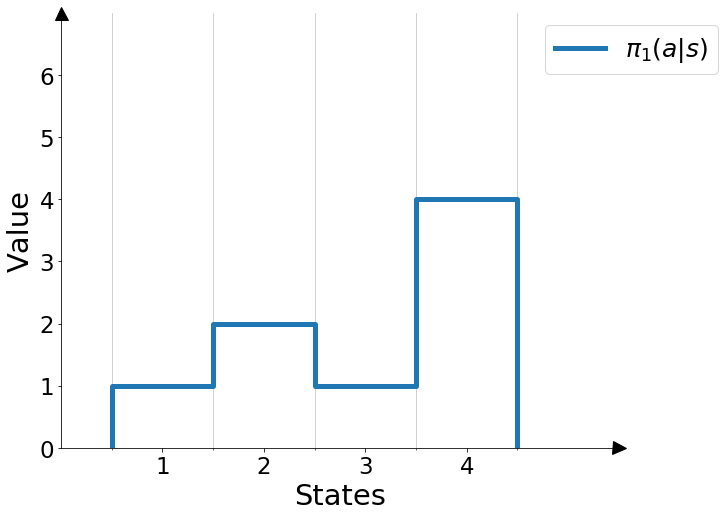
\includegraphics[width=8cm]{./images/pi1.png}
\centering
\end{figure}

\end{frame}


\begin{frame}{Control}

Improving a policy

\begin{figure}[t]
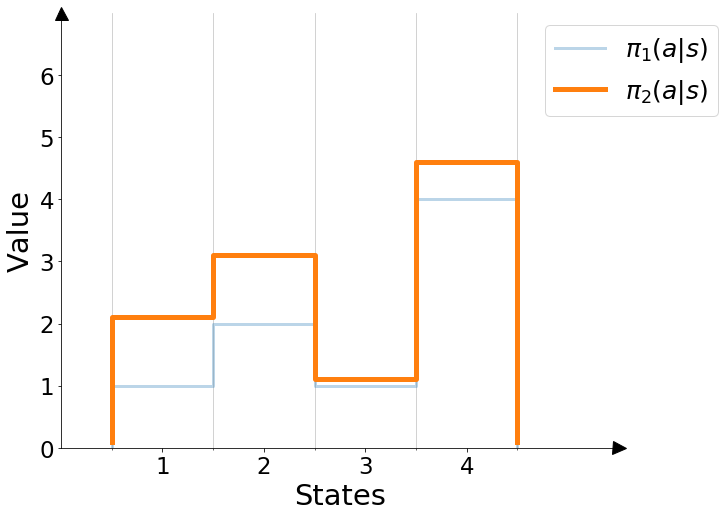
\includegraphics[width=8cm]{./images/pi2.png}
\centering
\end{figure}

\end{frame}

\begin{frame}{Control}

Improving a policy

\begin{figure}[t]
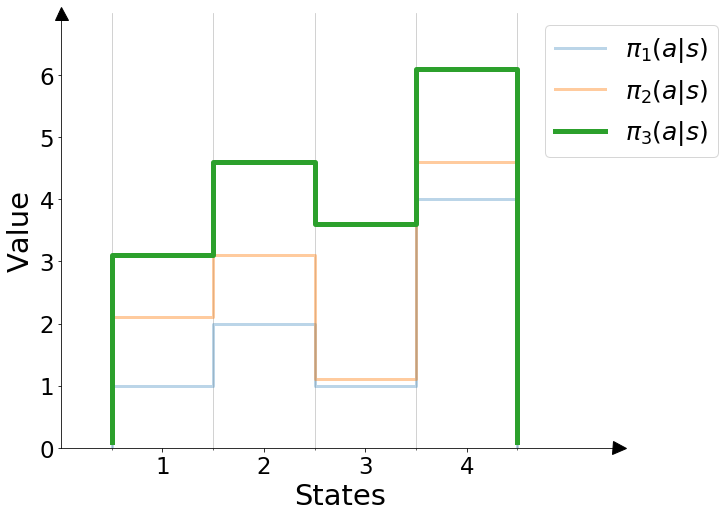
\includegraphics[width=8cm]{./images/pi3.png}
\centering
\end{figure}

\end{frame}


%============================================================================
\begin{frame}{Policy Evaluation}
\section{Policy Evaluation}

\textcolor{RoyalBlue}{Evaluating} a policy $\pi$ means computing its state-value function (or state-action value function).

\vspace{2mm}

If the environment dynamic is completely known, this problem is reduced to find the solution to a set of $\mathcal{|S|}$ linear equations:



\begin{align*}
    V^{\pi}(s)& = \mathds{E} \bigg[\sum_{k}^{\infty}\gamma^{k} r_{t+k+1} \: \bigg| \: s_t=s,\pi \bigg] \\
		   & = \sum_a \pi(a|s) \sum_{s_{t+1}} p(s_{t+1}|s,a)\big[r + \gamma V^{\pi}({s_{t+1}}) \big] 
\end{align*}

\end{frame}


%============================================================================
\begin{frame}{Iterative Policy Evaluation}

Since the above computation is complex, we can compute the value function for a given policy \textcolor{RoyalBlue}{iteratively}:
\begin{itemize}
    \item We choose $V^0$ arbitrarily
    \item We compute a sequence of improved approximations $V^1, V^2, V^3 ...$  by applying the Bellman equation to the previous estimate:
\end{itemize}

\begin{align*}
    &V^{k+1}(s) = \mathds{E} \bigg[\sum_{k}^{\infty}\gamma^{k} r_{t+k+1} \: \bigg| \: s_t=s,\pi \bigg] \\
		   & = \sum_a \pi(a|s) \sum_{s_{t+1}} p(s_{t+1}|s,a)\big[r + \gamma V^{k}(s_{t+1}) \big] \; \text{for each } s \in S
\end{align*}

The sequence $\{V_k\}$ is proven to converge to $V_{\pi}$ as $k \rightarrow \infty $.

\end{frame}



\begin{frame}{Gridworld}

\begin{itemize}
    \item $\mathcal{S}$: 16 states, with 2 terminal ones (0 nd 16)
    \item $\mathcal{A}$: Four possible actions: $\uparrow$ (up), $\downarrow$ (down), $\leftarrow$ (left), $\rightarrow$ (right)
\item $\mathcal{R}(s,a)$: $r_t = -1$ for every step in a non-terminal state, 0 in both terminal states
\end{itemize}

\begin{figure}[t]
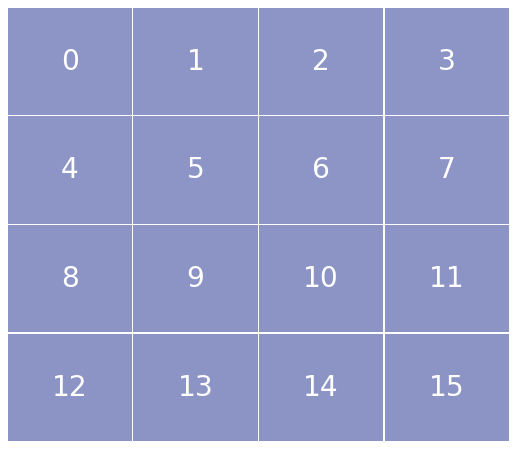
\includegraphics[width=4.5cm]{./images/GridWorld.png}
\centering
\end{figure}


\end{frame}


\begin{frame}{Iterative Policy Evaluation}

\begin{small}

We want to evaluate the \textcolor{RoyalBlue}{uniform random policy}, which has probability $0.25$ of taking each of the 4 possible actions.

\begin{align*}
    V(s_{t+1}) := \sum_a \textcolor{blue}{\pi(a|s)} \sum_{s_{t+1}} \sum_r p(s_{t+1},r|s,a)\Big[\textcolor{orange}{r+\gamma\:V(s_{t+1})}\Big]
\end{align*}
\end{small}
\begin{footnotesize}
\begin{align*}
    \textcolor{blue}{0.25}\cdot(\textcolor{orange}{-1 + 0}) + \textcolor{blue}{0.25}\cdot(\textcolor{orange}{-1+0}) + \textcolor{blue}{0.25}\cdot(\textcolor{orange}{-1+0})+ \textcolor{blue}{0.25}\cdot(\textcolor{orange}{-1+0}) = -1
\end{align*}

\end{footnotesize}

\begin{figure}[t]
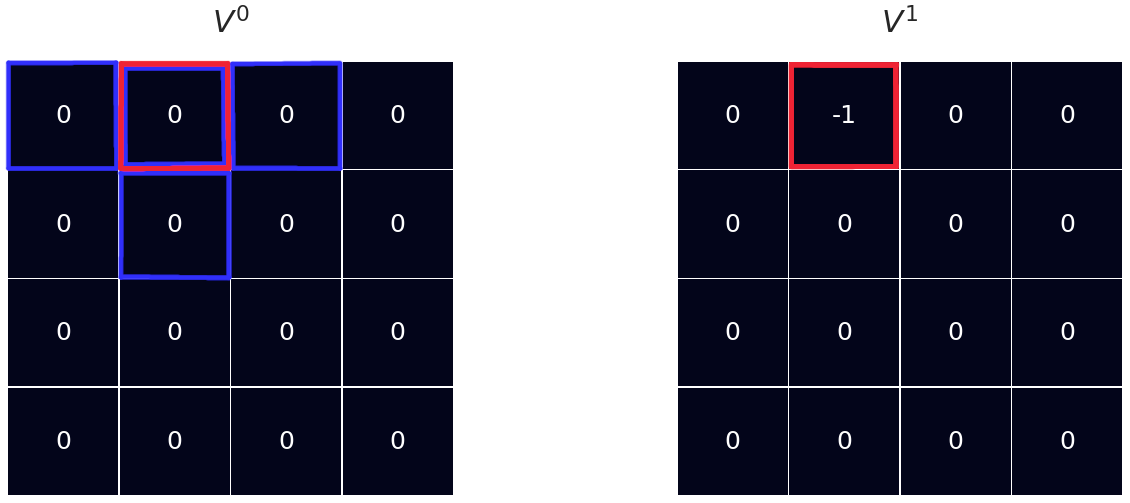
\includegraphics[width=9.7cm]{./images/step00.png}
\centering
\end{figure}

\end{frame}




\begin{frame}{Iterative Policy Evaluation}

\begin{small}

We want to evaluate the \textcolor{RoyalBlue}{uniform random policy}, which has probability $0.25$ of taking each of the 4 possible actions.

\begin{align*}
    V(s_{t+1}) := \sum_a \textcolor{blue}{\pi(a|s)} \sum_{s_{t+1}} \sum_r p(s_{t+1},r|s,a)\Big[\textcolor{orange}{r+\gamma\:V(s_{t+1})}\Big]
\end{align*}
\end{small}
\begin{footnotesize}
\begin{align*}
    \textcolor{blue}{0.25}\cdot(\textcolor{orange}{-1 + 0}) + \textcolor{blue}{0.25}\cdot(\textcolor{orange}{-1+0}) + \textcolor{blue}{0.25}\cdot(\textcolor{orange}{-1+0})+ \textcolor{blue}{0.25}\cdot(\textcolor{orange}{-1+0}) = -1
\end{align*}

\end{footnotesize}

\begin{figure}[t]
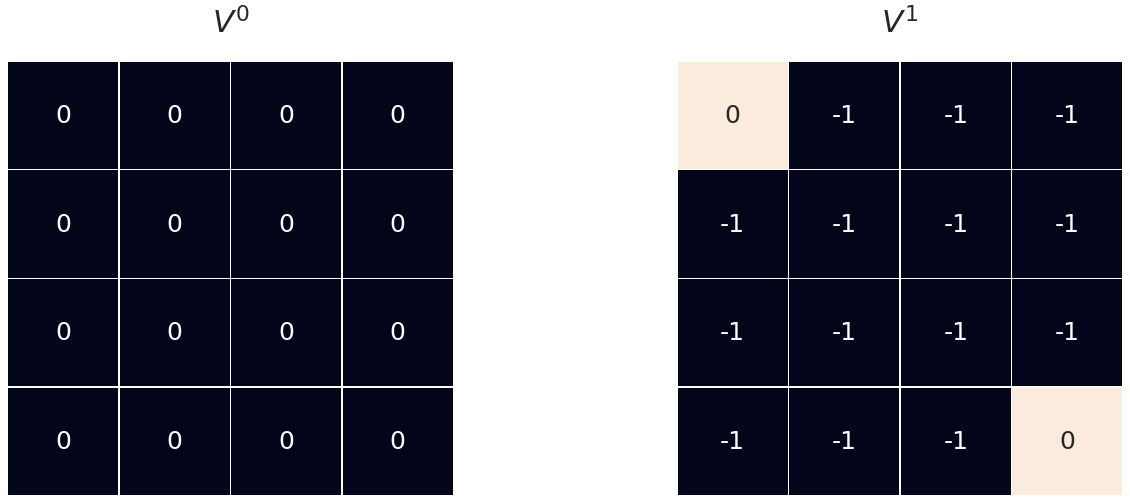
\includegraphics[width=9.7cm]{./images/step0.png}
\centering
\end{figure}

\end{frame}



\begin{frame}{Iterative Policy Evaluation}

\begin{small}
\begin{align*}
    V(s_{t+1}) := \sum_a \textcolor{blue}{\pi(a|s)} \sum_{s_{t+1}} \sum_r p(s_{t+1},r|s,a)\Big[\textcolor{orange}{r+\gamma\:V(s_{t+1})}\Big]
\end{align*}

\end{small}
\begin{figure}[t]
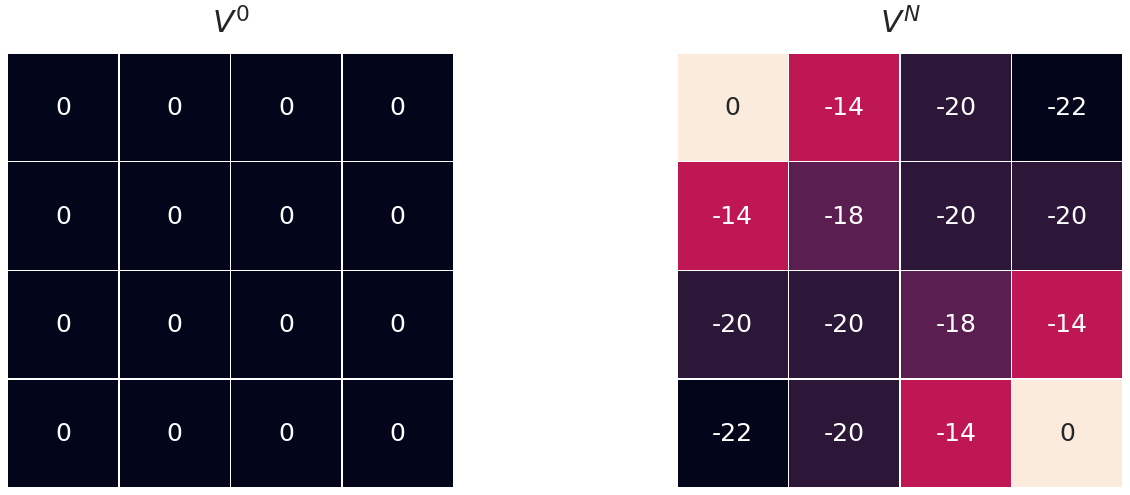
\includegraphics[width=9.7cm]{./images/stepn.png}
\centering
\end{figure}

\end{frame}



\begin{frame}{Iterative Policy Evaluation}


\begin{algorithm}[H]
\caption{Iterative Policy Evaluation}

%\SetAlgoLined

\vspace{1mm}
Input the policy to evaluate $\pi$

\vspace{0.5mm}

Define threshold for accuracy $\theta$

\vspace{0.5mm}

Initialize $V(s)$, for all $s \in \mathcal{S}$ arbitrarily, except V(terminal) = 0

\vspace{4mm}

$\Delta \leftarrow 0$
 

 \textbf{\text{while}} \text{True} 

 \hspace{5mm}  \textbf{\text{for}} \text{each} $s \in S$
   
   \vspace{0.5mm}
   
   \hspace{15mm} $v \leftarrow V(s)$
   
   \vspace{0.7mm}
   
   \hspace{15mm} $V(s) \leftarrow \sum_{a} \pi(a|s) \sum_{s^{\prime}, r} p(s^{\prime}, r | s, a)[r + \gamma V(s^{\prime})]$
   
   \vspace{0.7mm}
   
   \hspace{15mm} $\Delta \leftarrow \max(\Delta, |v - V(s)|)$
   
   \vspace{0.5mm}
   
   \hspace{5mm} if $\Delta < \theta$ return V
   \vspace{1mm}
   

\end{algorithm}

\end{frame}

%============================================================================
\begin{frame}{Policy Improvement}

How can we improve our policy once we know its value function?

\begin{align*}
    &Q_{\pi}(s,a) = \mathds{E} \bigg[\sum_{k}^{\infty}\gamma^{k} r_{t+k+1} \: \bigg| \: s_t=s, a_t=a,\pi \bigg] \\
		   & =  \sum_{s_{t+1}} p(s_{t+1}|s,a)\big[r + \gamma V^{k}(s_{t+1}) \big]
\end{align*}

\end{frame}

\begin{frame}{Policy Improvement}


\begin{block}{Policy Improvement Theorem}
Given any pair of deterministic policies $\pi$ and $\pi^{\prime}$ such that:
\begin{align*}
Q^{\pi}(s, \pi^{\prime}(s)) \geq Q^{\pi}(s, \pi(s))
\end{align*}

Which is the same as:
\begin{align*}
Q^{\pi}(s, \pi^{\prime}(s)) \geq V^{\pi}(s)
\end{align*}
Then policy $\pi^{\prime}$ is as good as or better than $\pi$:
\begin{align*}
    V^{\pi^{\prime}}(s) \geq V^{\pi}(s)
\end{align*}
\end{block}

\hspace{1mm}

The new policy $\pi^{\prime}$ can be found as:
\begin{align*}
    \pi^{\prime} = \argmax_{a \in A} Q^{\pi}(s,a)
\end{align*}

\end{frame}

\begin{frame}{Policy Iteration}
\section{Policy Iteration}

\begin{align*}
\pi_0 \; \overset{E}{\longrightarrow} \; V^{\pi_0} \overset{I}\longrightarrow \pi_1 \overset{E}\longrightarrow V^{\pi_1} \overset{I}\longrightarrow . . . \overset{I}\longrightarrow \pi_{*} \overset{E}\longrightarrow V^{\pi_*}
\end{align*}

Since a finite MDP has only a finite number of policies, this process must converge to an \textcolor{RoyalBlue}{optimal policy} in a finite number of iterations.

\end{frame}

\begin{frame}{Policy Iteration}

\begin{algorithm}[H]
\caption{Policy Iteration for estimating $\pi \sim \pi^{*}$}

\vspace{1mm}

%\SetAlgoLined
1) \textbf{\text{Initialization}}

Initialize $V(s) and \pi(s)$ \text{ arbitrarily for all } $s \in S$
\vspace{3mm}


2) \textbf{\text{Policy Evaluation Step}} (Algorithm 1)
\vspace{3mm}

3) \textbf{\text{Policy Improvement Step:}}

\vspace{0.5mm}

\hspace{6mm}policy-stable $\leftarrow$ true 

\vspace{0.5mm}

 \hspace{5mm} \textbf{\text{for}} \text{each} $s \in \mathcal{S}$ \textbf{\text{do}} 
 
 \vspace{0.4mm}
 
 \hspace{11mm} old-action $\leftarrow \pi(s)$
 
 \vspace{0.5mm}
 
 \hspace{11mm} $\pi(s) \leftarrow \argmax_a \sum_{s_{t+1}} p(s_{t+1}|s,a) [r + \gamma V(s^{t+1})]$
 
 \vspace{0.5mm}
 
 \hspace{11mm} if old\text{-}action $\neq \pi(s)$, \text{policy-stable} $\leftarrow$ false
 
 \vspace{0.5mm}
 
 \hspace{6mm}if policy-stable = true then return $\pi \sim \pi^{*}$
 

\vspace{1mm}
\end{algorithm}

\end{frame}
%============================================================================
\begin{frame}{Value Iteration}

\textcolor{Maroon}{Drawback} of Policy Iteration: in each iteration we need to perform policy evaluation.

\vspace{2mm}

The policy evaluation step can be \textcolor{RoyalBlue}{truncated} without losing convergence guarantees.

\begin{align*}
    &V^{k+1}(s) = \max_a \;  \mathds{E} \bigg[\sum_{k}^{\infty}\gamma^{k} r_{t+k+1} \: \bigg| \: s_t=s, a_t = a \bigg] \\
		   & = \max_a \sum_{s_{t+1}} p(s_{t+1}|s,a)\big[r + \gamma V^{k}(s_{t+1}) \big] \; \text{for each } s \in S
\end{align*}


\end{frame}


\begin{frame}{Value Iteration}


\begin{algorithm}[H]
\caption{Value Iteration Algorithm}

%\SetAlgoLined

\vspace{1mm}

Define threshold for accuracy $\theta$

Initialize $V(s)$, for all $s \in \mathcal{S}$, arbitrarily

\vspace{4mm}

 $\Delta \leftarrow 0$

 \textbf{\text{while}} \text{True} \textbf{\text{do}}
 
 \vspace{0.5mm}
 
 \hspace{6mm} \textbf{\text{for}} \text{each} $s \in \mathcal{S}$ \textbf{\text{do}}
 
   
   \hspace{15mm} $v \leftarrow V(s)$
   
   \hspace{15mm} $V(s) \leftarrow \max_a \sum_{s_{t+1}}p(s_{t+1}|s,a)\Big[r+\gamma\:V(s_{t+1})\Big]$
   
   \hspace{15mm} $\Delta \leftarrow \max(\Delta, |v - V(s)|)$
   
   until $\Delta < \theta$

   \vspace{4mm}

   Output a deterministic policy $\pi \sim \pi^{*}$, such that:
   
   $\pi(s) \leftarrow \argmax_a \sum_{s_{t+1}}p(s_{t+1}|s,a)\Big[r+\gamma\:V(s_{t+1})\Big]$
   

\end{algorithm}

\end{frame}


%============================================================================
\begin{frame}{Generalised Policy Iteration}
\section{Generalised Policy Iteration}

We define generalized policy iteration as the \textcolor{RoyalBlue}{alternative execution of policy evaluation and policy improvement}, regardless of the granularity of the two processes.

\hspace{2mm}

This process stabilizes only when we found a policy that is greedy with respect to its own value function.

\end{frame}


\begin{frame}{Final Slide!}
	\begin{takeaway}{Lecture Takeaway}
		\begin{enumerate}
			\item Given $p(s^{\prime}|s,a)$ we can find the optimal policy mathematically
			\item But better use Dynamic Programming algorithms
			\item It works by alternating the tasks of Policy Evaluation and Control
		\end{enumerate}
	\end{takeaway}
\end{frame}


\end{document}
